Danas je prva asocijacija na spomen napredne obrade slike umjetna inteligencija i duboke neuronske mreže.
Uz to, tehnika konvolucije se pokazala daleko najprimjerenija za rješavanje istih problema. \\
Problem koji se javlja s rezultantnim modelima dubokih neuronskih mreža je što su gotovo uvijek nerazumljivi i rade kao \emph{crne kutije}.
Točnije, ljudima je teško razumjeti i objasniti kako je mreža došla do izlaza kojeg je stvorila. \\
Velika prednost modela, nastalim genetskim algoritmom je što je izlazni model jasno razumljiv (Slika ~\ref{fig:gen_alg_tree_1}). \\
Genetsko programiranje se i ranije koristilo kao način obrade slike uz razlike kao što su (\cite{cgp_image_processing}):
\begin{itemize}
	\item jednostavnija arhitektura npr. stablo
	\item manji skup funkcija
\end{itemize}

\begin{figure}
	\centering
	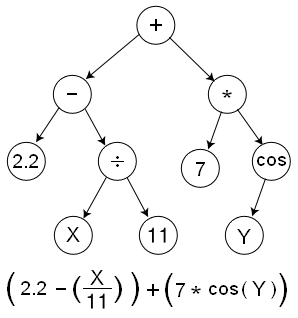
\includegraphics[width=0.6\linewidth]{Illustrations/Genetic_Program_Tree.png}
	\caption{Rezultantno stablo nastalo radom genetskog algoritma}
	\label{fig:gen_alg_tree_1}
\end{figure}

Ovaj rad, baviti će se uporabom \emph{Kartezijskog genetskog programiranja} (\emph{CGP}), čija je arhitektura inspirirana dubokim neuronskim mrežama, u svrhu obrade i analize slike. \\
U nastavku rada, ukratko ću objasniti što je genetsko programiranje te kako radi.
Detaljno ću predstaviti \emph{CGP} kao tehniku genetskog programiranja, izraziti prednosti nad klasičnim metodama te predstaviti način na koji sam implementirao konvolucijske tehnike u svrhu provedbe eksperimenata.
Predstaviti ću sve eksperimente koje sam proveo, prikazati i objasniti rezultate te usporediti dobivene rezultate s željenim.
Na kraju, okušati ću se u korištenju \emph{CGP-a} kao metode izrade \emph{autoencoder-a} te ću ispitati ograničenja korištenja genetskog programiranja kao prikladne tehnike za generiranje uzoraka zadane raspodjele.

Cilj rada je dati čitatelju ideju o radu i performansama \emph{CGP-a} kroz provedene eksperimente te poslužiti kao inspiracija i početka točka za buduće eksperimente.
